\section{\texorpdfstring{$*$}{*}应用：球面映射}
\sourcepage{135--136}
本节给出同调论对几何与拓扑经典问题的若干应用。下一节的著名 Lefschetz 不动点定理将推广这里的结果。

\entry{定义}{2.9.1}设 $n\geq1$，$f:S^n\to S^n$ 连续。若 $\alpha$ 为无限循环群 $H_n(S^n)$ 的两个生成元之一，则对某个整数 $d$，$f_*(\alpha)=d\alpha$。因为 $f_*(-\alpha)=d(-\alpha)$，$d$ 与生成元选择无关，称为 $f$ 的\textbf{映射度}（degree），记为 $\deg f$。

\entry{引理}{2.9.2}映射度满足：
\begin{enumerate}[label=(\arabic*)]
\item 若 $f\simeq g$，则 $\deg f=\deg g$。
\item 若 $f$ 能扩张为连续映射 $\widehat f:B^{n+1}\to S^n$，则 $\deg f=0$。
\item 恒等映射的映射度为 $1$。
\item $\deg(f\circ g)=(\deg f)(\deg g)$。
\end{enumerate}
\noindent\textbf{证明：}(1) 由定理 2.7.5。(2) 中 $f_*$ 为复合
\[
H_n(S^n)\xrightarrow{j_*}H_n(B^{n+1})\xrightarrow{\widehat f_*}H_n(S^n),
\]
其中 $j$ 为包含。球无环，所以复合为零。(3)、(4) 直接由定理 2.6.2 得到。\hfill$\square$

\entry{定理}{2.9.3}不存在收缩映射 $r:B^{n+1}\to S^n$。

\noindent\textbf{证明：}恒等映射的映射度为 $1$。若有收缩映射，它就是恒等映射到球的扩张，由引理 (2)，恒等映射的度又为 $0$，矛盾。\hfill$\square$

\entry{定理}{2.9.4（Brouwer 不动点定理）}若 $\varphi:B^n\to B^n$ 连续，则存在 $x\in B^n$，使 $\varphi(x)=x$。

\noindent\textbf{证明：}假设没有不动点，则可定义
\[
h:B^n\to S^{n-1},\qquad h(x)=\frac{x-\varphi(x)}{\|x-\varphi(x)\|}.
\]
令 $f$ 为其在边界球面上的限制，由引理 (2)，$\deg f=0$。另一方面，定义
\[
H(u,t)=\frac{u-t\varphi(u)}{\|u-t\varphi(u)\|}.
\]
当 $t=1$ 时，分母由无不动点假设非零；当 $t<1$ 时，$\|u\|=1$，而 $\|t\varphi(u)\|\leq t<1$，分母仍非零。此同伦连接恒等映射和 $f$，故 $\deg f=1$，矛盾。\translatornote{由于前面只对正维球面定义映射度，此证明直接适用于 $n\geq2$；$n=1$ 可由介值定理证明，$n=0$ 平凡。}\hfill$\square$

\entry{定义}{2.9.5}\textbf{对径映射}（antipodal map）$a:S^n\to S^n$ 定义为 $a(x)=-x$。

后续应用需要证明其映射度为 $(-1)^{n+1}$。这里给直接证明，下一节及第 4.4 节还会给出其他证明。关键是下面的引理。

\entry{引理}{2.9.6}反射映射 $\rho:S^n\to S^n$，
\[
\rho(x_1,\ldots,x_n,x_{n+1})=(x_1,\ldots,x_n,-x_{n+1}),
\]
的映射度为 $-1$。

反射在球面每点处反转切平面的定向，这或许直观清楚，但仍须依定义 2.9.1 证明。先定义所需的三角剖分。

\sourcepage{137--138}
\entry{定义}{2.9.7}空间 $X$ 的一个\textbf{三角剖分}（triangulation）是复形 $L$ 连同同胚 $h:|L|\to X$。若存在这样的剖分，称 $X$ \textbf{可三角剖分}（triangulable）。

\noindent\textbf{引理 2.9.6 的证明：第一步。}构造 $S^n$ 的 $n$ 维三角剖分，使反射对应于该复形到自身的单纯映射。

设有限复形 $K\subset\R^N\times\{0\}$，取 $w_0=(0,\ldots,0,1)$、$w_1=(0,\ldots,0,-1)$，令悬挂 $S(K)=(w_0*K)\cup(w_1*K)$。令 $r$ 交换两个锥顶并固定 $K$ 的各顶点。要构造 $n-1$ 维复形 $K$ 及同胚 $k:|S(K)|\to S^n$，使 $\rho k=kr$。

取 $S^{n-1}$ 的任意 $n-1$ 维三角剖分 $h:|K|\to S^{n-1}$。若 $y=(1-t)x+tw_0$，定义 $k(y)=(\sqrt{1-t^2}\,h(x),t)$；若 $y=(1-t)x+tw_1$，定义 $k(y)=(\sqrt{1-t^2}\,h(x),-t)$，见图 2.9.1。
\begin{center}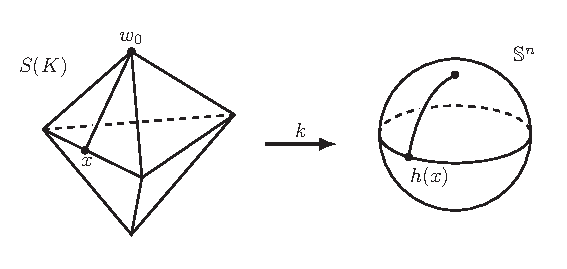
\includegraphics[width=101mm]{figures/2-9-1.pdf}\\图 2.9.1\end{center}
容易验证 $k$ 为同胚。又因为 $r((1-t)x+tw_0)=(1-t)x+tw_1$，所以 $\rho k=kr$。

\textbf{第二步。}只需证明 $r$ 对最高维同调作用为乘以 $-1$。设 $z$ 为 $S(K)$ 的 $n$ 维闭链，因 $\dim K=n-1=m$，可写成 $z=[w_0,c_m]+[w_1,d_m]$。若 $n>1$，
\[
0=\partial z=c_m-[w_0,\partial c_m]+d_m-[w_1,\partial d_m].
\]
限制到 $K$ 得 $c_m+d_m=0$，故 $z=[w_0,c_m]-[w_1,c_m]$。于是 $r_\#z=[w_1,c_m]-[w_0,c_m]=-z$。$n=1$ 的计算类似。\hfill$\square$

\entry{定理}{2.9.8}对 $n\geq1$，对径映射的映射度为 $(-1)^{n+1}$。

\noindent\textbf{证明：}任意坐标反射 $\rho_i$ 的度也为 $-1$。事实上，交换第 $i$、第 $n+1$ 坐标的同胚 $h$ 满足 $\rho_i=h^{-1}\rho h$，所以
\[
\deg\rho_i=(\deg h^{-1})(\deg\rho)(\deg h)
=\deg(h^{-1}h)\deg\rho=-1.
\]
而 $a=\rho_1\rho_2\cdots\rho_{n+1}$，故得到结论。\hfill$\square$

\entry{定理}{2.9.9}若 $h:S^n\to S^n$ 的映射度不等于 $(-1)^{n+1}$，则它有不动点。

\noindent\textbf{证明：}反设没有不动点。将 $h(x)$ 沿最短大圆弧移动到 $-x$，得到 $h\simeq a$，故度为 $(-1)^{n+1}$，矛盾。具体同伦为
\[
H(x,t)=\frac{(1-t)h(x)-tx}{\|(1-t)h(x)-tx\|}.
\]
若分母为零，则 $(1-t)h(x)=tx$，取范数得 $1-t=t$，即 $t=1/2$，进而 $h(x)=x$，矛盾。\hfill$\square$

\sourcepage{139}
\entry{定理}{2.9.10}若 $h:S^n\to S^n$ 的度不等于 $1$，则它将某点映到该点的对径点。

\noindent\textbf{证明：}$ah$ 的度不等于 $(-1)^{n+1}$，故有不动点 $x$。于是 $a(h(x))=x$，即 $h(x)=-x$。\hfill$\square$

\entry{推论}{2.9.11}球面 $S^n$ 存在处处非零的切向量场，当且仅当 $n$ 为奇数。

\noindent\textbf{证明：}若 $n=2k-1$，对 $x\in S^n\subset\R^{2k}$ 定义
\[
v(x)=(-x_2,x_1,-x_4,x_3,\ldots,-x_{2k},x_{2k-1}).
\]
它与 $x$ 垂直，故切于球面，且 $\|v(x)\|=\|x\|=1$，处处非零。

反过来，若有处处非零的切向量场 $w$，则 $h(x)=w(x)/\|w(x)\|$ 为球面到自身的映射。因 $w(x)\perp x$，既不可能 $h(x)=x$，也不可能 $h(x)=-x$。由定理 2.9.9、2.9.10，分别得 $\deg h=(-1)^{n+1}$ 和 $\deg h=1$，故 $n$ 为奇数。\hfill$\square$

习题 2 要求证明代数基本定理，为完整起见陈述如下。

\entry{定理}{2.9.12（代数基本定理）}每个实或复系数多项式 $z^n+a_{n-1}z^{n-1}+\cdots+a_1z+a_0$（$n\geq1$）在复平面中都有根。

\sourcepage{140--141}
\subsection*{习题}
\begin{enumerate}
\item \begin{enumerate}[label=(\alph*)]
\item 设 $K$ 为图 2.9.2 的正方形边界复形，$\operatorname{sd}K$ 为第一次重心剖分。单纯映射 $f:\operatorname{sd}K\to K$ 由 $f(a_i)=a_{2i}$ 给定，下标必要时模 $8$。证明其映射度为 $2$。
\begin{center}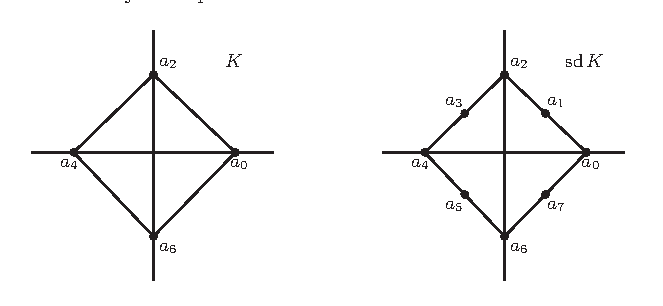
\includegraphics[width=117mm]{figures/2-9-2.pdf}\\图 2.9.2\end{center}
\item 将 $S^1$ 视为单位模复数集，证明 $h(z)=z^2$ 的度为 $2$。［提示：通过径向投影，它给出 $|K|$ 到自身的映射，与 (a) 的 $f$ 同伦。］
\item 对任意正整数 $n$，证明 $k(z)=z^n$ 的度为 $n$。
\end{enumerate}
\item 用习题 1 按下列步骤证明代数基本定理。令 $S_c$ 为复平面中圆周 $|z|=c$。假定给定多项式在闭圆盘 $|z|\leq c$ 中没有根，定义 $h:S_c\to\mathbb C\setminus\{0\}$ 为 $h(z)=z^n+a_{n-1}z^{n-1}+\cdots+a_0$。
\begin{enumerate}[label=(\alph*)]
\item 证明 $h_*$ 为零同态。
\item 证明当 $c$ 足够大时，$h$ 同伦于 $k(z)=z^n$。［提示：取 $F(z,t)=z^n+t(a_{n-1}z^{n-1}+\cdots+a_0)$。］
\item 导出矛盾。
\end{enumerate}
\item 按下列步骤证明反射映射引理证明中第一步的 $k$ 为同胚。\translatornote{原文误引为定理 2.9.8 的证明，实际在引理 2.9.6 的证明中。}
\begin{enumerate}[label=(\alph*)]
\item 证明映射 $p:|K|\times[-1,1]\to|S(K)|$ 与 $q:|K|\times[-1,1]\to S^n$ 均为商映射，其中
\[
p(x,t)=\begin{cases}(1-t)x+tw_0,&t\geq0,\\(1+t)x-tw_1,&t<0,\end{cases}
\qquad q(x,t)=(\sqrt{1-t^2}\,h(x),t).
\]
\item 证明 $p,q$ 诱导同胚 $k$。
\end{enumerate}
\item 证明习题 1(c) 对 $n\leq0$ 的整数也成立。
\item 参照习题 1(b)，设 $m$ 为任意复常数，证明函数 $f(z)=(z+m)^2$ 的度为 $2$。［提示：用同伦论证。］\translatornote{原题未说明此函数的定义域和值域。它一般不是 $S^1\to S^1$ 的映射；若理解为在充分大圆周上归一化所得的圆周映射，其度为 $2$。不能对任意 $m$ 直接在单位圆周上使用这一断言。}
\end{enumerate}
